\chapter{Introduction}
\markright{Introduction} % new right header
%======================================================================
\section{Inorganic Chemistry}
%======================================================================

Common distinctions split most chemical compounds into one of two categories: organic and inorganic. Organic molecules contain carbon and hydrogen, with or without additional nitrogen, oxygen, phosphorus, sulfur, and the halides. Inorganic chemistry is, therefore, considered to be the remainder of the molecules possible. While they may include come aspect of organic chemistry (especially in organometallic molecules), the main structural motif or reactive center is a non-organic feature. These inorganic compounds can range from compounds such as lithium or grignard reagents with significant organic influence, to metallic alloys or mineral compounds. With such a wide range of possibilities, inorganic chemistry has many facets. A widely active research area is the development and testing of transition metal complexes for catalytic, photo-physical, biochemical or manufacturing uses.

%======================================================================
\section{Photochemistry \& Catalysis}
%======================================================================

A report of the first synthesized organometallic complex was published by Zeise in 1831\autocite{zeise1831}. To form what is now known as Zeise's salt, \ce{K[PtCl3(C2H4)]*H2O}, he mixed platinum chloride with ethanol, followed by a reaction with potassium chloride\autocite{hunt1984}. After some controversy to the composition of this, it was confirmed by Griess and Martius\autocite{griess1861}, and later expanded upon by Birnbaum\autocite{birnbaum1868}. 

The field of organometallics was expanded greatly by Frankland\autocite{hunt1984}, and many of his complexes were catalytically active. Further development of this new type of chemistry quickly led to useful catalysts for the conversion of petroleum products or the production or destruction of other chemicals to be developed using nearly all of the transition metals. These catalysts take all forms, from simple olefin and halide compounds to multi-metallic complexes with large organic ligands.

Some of the most interesting organometallic catalysts since the late 1990s have been the development of earth metal pincer complexes to replace noble metal or early transition metal catalysts, which are often more toxic or expensive to produce. Brookhart and Gibson published a series of papers\autocite{small1998a, small1998b, britovsek1998, britovsek1999} on the use of iron and cobalt with bis(imino)pyridine ligands to perform ethylene polymerization at rates exceeding those of similar noble metal complexes and metallocenes\autocite{gibson2007}. The role of the ligand in the mechanism is still up for debate, but many modified systems have been synthesized and tested since the first work was published\autocite{boudier2014}.

Many of these types of pincer complexes are photochemically active. In transition metal complexes, the interaction between the metal atom(s) and the ligands can cause significant electron mobility upon the absorption of incident photons. The metal atom's \textit{d} orbitals typically lie at or near the \gls{ac.homo} energy, while the ligands often have low energy anti-bonding orbitals ($\pi^\ast$) at the \gls{ac.lumo} levels. When a photon is absorbed and is promoted from the ground state to the excited state, that state is geographically removed from the metal centre, this motion of the electron is labelled a \gls{ac.mlct}. Formally, the metal atom is oxidized by the photons, this oxidation allows for redox reactivity at the metal centre for as long as the electron remains removed to the ligand. Relaxation (through photon emission via fluorescence or phosphorescence, or via vibrational or other motion processes) can return the electron to the metal to reform the ground electronic state. 



%======================================================================
\section{Rhenium}
%======================================================================

\todo{Rewrite to more verbose}Rhenium compounds display a broad scope of applications ranging from catalysis\autocite{dudle2011, jain2008, kuninobu2011} to radiopharmaceutical applications\autocite{bartholoma2009, schibli2002}, as well as possessing interesting fundamental photophysical properties\autocite{coogan2009}. Since the mid-1970's, complexes containing the $\alpha$-diimine \ce{Re^I} tricarbonyl core have attracted a great deal of attention due to their attractive photochemical properties with pseudo-octahedral \textit{fac}-\ce{[L2Re(CO)3X]} and \textit{fac}-\ce{[L2(L$'$)Re(CO)3]+} complexes being the dominant species\autocite{giordano1979, fredericks1979, sacksteder1990, caspar1983, yam2001, feliz1998, ruiz1996, lin1992, hino1992, walters2002, striplin2001}. A large family of compounds with these formulations have been accessed by the addition of chelating diimine $\sigma$-donor ligands to \ce{[Re(CO)5X]} with the quantitative replacement of two \textit{cis} carbonyls in the \ce{Re^I} starting material\autocite{giordano1979, martin2011, abel1959, kirkham1965, zingales1967, gamelin1994, marti2005, morse1976, giordano1978}. Significantly, these reactions form only bidentate coordinated ligands with \textit{facial} tricarbonyl isomers as products even when a potentially tridentate $\sigma$-donor, such as bis(imino)pyridine or 2,2':6',2''-terpyridine are employed in the reaction (Figure \ref{fig.terdentateligands})\autocite{granifo1999, orrell1997, abel1993}. These robust species have been examined for potential applications in organic light-emitting diodes (OLEDs)\autocite{gong1998}, chemosensors and biotechnology probes\autocite{lo2010, lin2007, slone1995, beer1999, beer2003}, fluorescence microscopy imaging of cells\autocite{lo2010, amoroso2008, amoroso2007}, and the photochemical reduction of \ce{CO2} to CO\autocite{hawecker1983, hawecker1986, takeda2010, christensen1992, sullivan1985}. Among the key photophysical features of these $\alpha$-diimine \ce{Re^I} compounds is the electron transfer capability of this system and the interplay between the Re center and the well-known non-innocent redox-activity of the ligands\autocite{caulton2012}.

\begin{figure}[!htbp]
 \begin{center}
  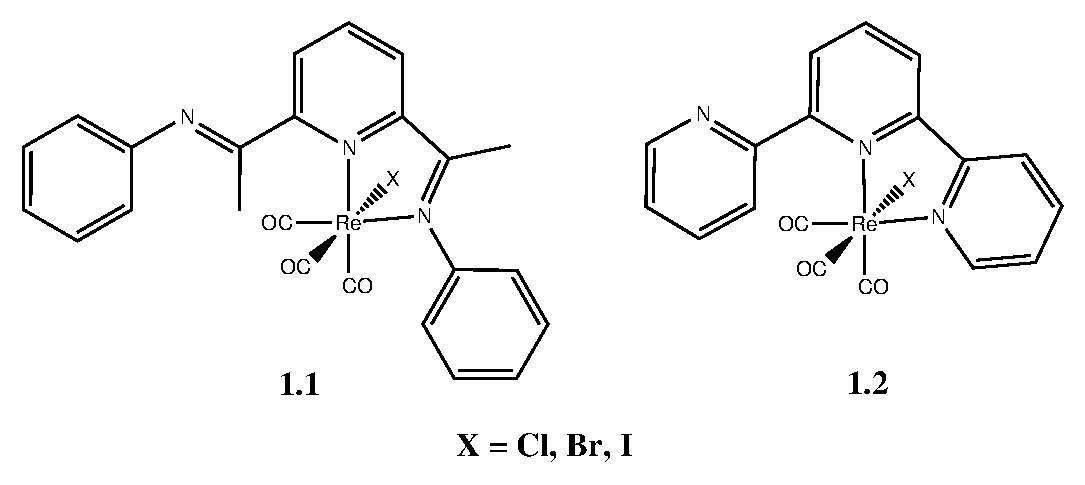
\includegraphics[clip=true, width=110mm]{images/terdentateligands.eps}
 \end{center}
\caption[Two common bidentate complexes using terdentate ligands]{Two common \textit{fac}-\ce{[L2Re(CO)3X]} complexes with terdentate $\sigma$-donor ligands: L = bis(imino)pyridine (\textbf{A}) and 2,2':6',2''-terpyridine (\textbf{B})}
\label{fig.terdentateligands}
\end{figure}

Further development of this chemistry has been restricted by the limited structural and electronic variability of the common pseudo-octahedral \textit{fac}-\ce{[L2ReX(CO)3]} (\ce{L2} = $\alpha$-diimine) products. While these systems continue to receive considerable attention, studies detailing the coordination chemistry of the meridionally-coordinated tridentate triimine \ce{Re^I} dicarbonyl core are quite limited\autocite{jurca2013}. For example, while \ce{$\kappa$^3(terpy)Re(CO)2Cl} was initially reported in 1988\autocite{juris1988}, closer analysis of the reported analytical data (including \textsuperscript{1}H NMR) indicate that this compound is more likely \ce{$\kappa$^2LRe(CO)3Cl}. A more recent report for this compound provides spectroscopic details of this species as well as the preliminary report for the generation of \ce{[$\kappa$^3(terpy)Re(CO)2L$'$]+} cations (L = \ce{PPh3}, \ce{PEt3}, \ce{NC5H5}, and \ce{NCCH3})\autocite{black2012}. Finally, the \textsuperscript{1}H NMR data for \ce{$\kappa$^3(terpy)Re(CO)2Br} has been reported\autocite{abel1993}.

In order to fully exploit the potential of this versatile family of compounds, the limits imposed by the bidentate coordination need to be addressed. Furthermore, it would appear that, on the basis of the tridentate ligands that have been investigated, the concerted effort to produce the tridentate species has been unsuccessful. Attracted by this challenge we sought to synthesize, crystallographically authenticate, and investigate the photophysical properties of low-valent rhenium pincer complexes displaying an N,N',N''-chelated terpyridine array. 

\todo{Take out spoilers}We recently reported the conversion of bidentate bis(imino)pyridine complexes 2,6-\{2,6-\ce{Me2C6H3N=CPh\}2(NC5H3)Re(CO)3X}  (X = Cl, Br) into tridentate pincer ligand compounds, 2,6-\{2,6-\ce{Me2C6H3N=CPh\}2(NC5H3)Re(CO)2X} (X = Cl, Br)\autocite{jurca2013}. This transformation was performed in the solid-state by controlled heating of these bidentate species above 200$^\circ$C in a tube furnace under a flow of nitrogen gas giving excellent yields ($\geq$~95\%). These compounds defined a new coordination environment for \ce{Re^I} carbonyl chemistry where the metal center is supported by a planar, tridentate pincer coordinated bis(imino)pyridine ligand. 

Complexes of 2,2':6',2''-terpyridine (terpy) are of interest due to the conceptual relationship to established bis(imino)pyridine compounds\autocite{russell2010, tondreau2012}. Herein, we provide rational synthetic procedures to these novel species as well as their characterization and analysis of their visible electronic transitions. These results will broaden the accessibility of such compounds for investigation and application. This report for the unconventional but accessible synthesis of tridentate pincer complexes promises to enhance the versatile chemistry of \ce{Re^I} and yield new venues for exploration.

This thesis will be a discussion of the development of chemistry of \ce{Re^I} complexes, their characterization, and comparison of structural and photo-physical properties to computed values. Further exploration of the \ce{CO2} reduction by photo-catalysis of these new complexes will be analyzed. This thesis will also take a more detailed look at specifics of the mechanisms proposed for current \ce{Re^I} diimine catalysts, and propose new geometries for prior mechanistic steps based on experimental, computational, and literature review work.

